% Drawing 154/03-5 -- folder 154, batch 03, archive page 50 (PDF page 51).
% Transcription: figures dans la moitié droite de la feuille : en haut, un cercle noir et gris traversé de courbes qui se croisent, deux points verts ; deux hexagones et un pentagone rouges, chacun traversé d'un segment vert joignant un sommet (point rouge) à un côté ; un hexagone rouge partagé par un segment vert, hachuré au crayon ; au bas, un réseau de droites rouges qui se croisent en losanges, parcouru d'une ligne brisée verte, et un faisceau rouge coupé par des segments verts en pointillé
% Kind: polygons with green segments; red line networks with green broken lines. Method 2 (schematic redraw from the facsimile). Status: partial.
% Notes: Right half of the sheet, read from the page view (positions to about 1-2 units). Top: a circle in black and grey crossed by intersecting curves, two green points on each side (four green points are visible), a thick black arc on its left. Two hexagons and a pentagon in red, each crossed by a green segment joining a vertex (red point) to a side; the lower hexagon has pencil lines inside and green arrows. Foot: a network of red lines crossing in lozenges, run through by a green zigzag line with two red points and a yellow dotted line; and to its right a red pencil of lines cut by a green broken line, a red cross at its end. The crossing curves in the circle are schematic. Still differs from the facsimile: The crossing curves in the circle are schematic.
% Coordinates: 1 unit = 1 mm = 1/100 of the crop width (bbox in page fractions: [0.556, 0.092, 0.955, 0.521]).
% Redrawn by Claude (claude-opus-5-5), issue #73, 2026-11-07; not checked by a human; not compiled (no TeX in the session).
% Revised by Claude (claude-opus-5-5) 2026-11-09 (issue #128) after Michel's check: vertices snapped to exact intersections (drawn points on their lines, meeting ends on the stroke they meet, near-concurrent lines through one computed point, curve ends on their rim); labels at \small as in folder 80 batch 3. Status: partial.
% Rights: reproduces part of the work -- behind RENDER_TRANSCRIPTS, never published by itself.
\documentclass[tikz,border=3pt]{standalone}
\usepackage{amsmath,amssymb}
\usetikzlibrary{patterns,arrows.meta}
\tikzset{Or/.style={orange!90!black}, Ye/.style={yellow!80!orange}, Lg/.style={green!60!black!70}, Dg/.style={green!45!black}, Br/.style={brown!80!black}, Rd/.style={red!85!black}, Bl/.style={blue!70!black}, Gy/.style={black!40}, pencil/.style={black!45}, struck/.style={black!35}, mark/.style={circle,draw,inner sep=1.3pt}, pt/.style={circle,fill,inner sep=0.9pt}, opt/.style={circle,draw,fill=white,inner sep=1.1pt}}
\begin{document}
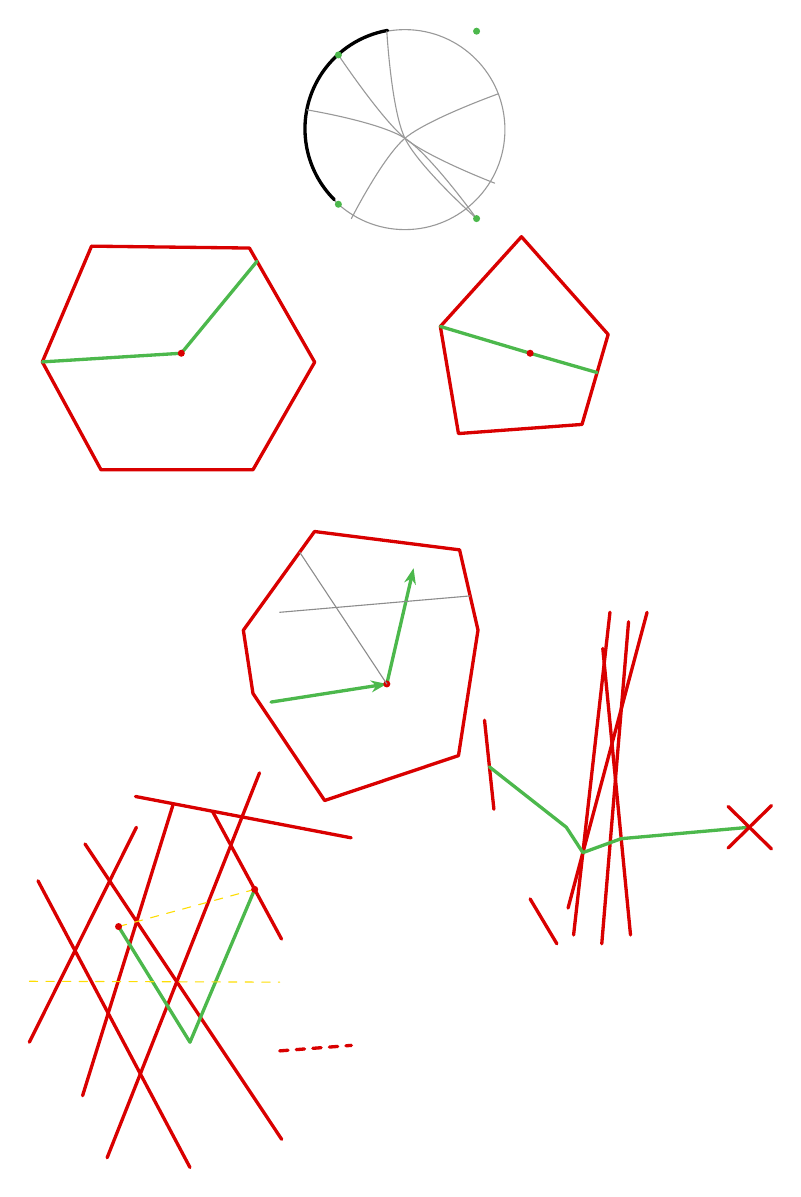
\begin{tikzpicture}[x=1mm,y=1mm,line cap=round,line join=round,font=\scriptsize]
\draw[Gy] (50,-18.2) circle[radius=12.7];
\draw[very thick] (47.8,-5.6) arc[start angle=100, end angle=225, x radius=12.7, y radius=12.7];
\draw[Gy] plot[smooth, tension=0.55] coordinates {(41.55,-8.72) (50,-19.3) (61.4,-25)};
\draw[Gy] plot[smooth, tension=0.55] coordinates {(43.2,-29.5) (50,-19.3) (61.86,-13.65)};
\draw[Gy] plot[smooth, tension=0.55] coordinates {(37.55,-15.69) (50,-19.3) (59.1,-29.5)};
\draw[Gy] plot[smooth, tension=0.55] coordinates {(47.7,-5.71) (50,-19.3) (59.1,-29.5)};
\node[pt,Lg] at (41.55,-8.72) {};
\node[pt,Lg] at (59.1,-5.7) {};
\node[pt,Lg] at (41.55,-27.68) {};
\node[pt,Lg] at (59.1,-29.5) {};
\draw[Rd,very thick] (3.95,-47.7) -- (10.2,-33) -- (30.25,-33.24) -- (38.54,-47.73) -- (30.7,-61.4) -- (11.4,-61.4) -- cycle;
\draw[Lg,very thick] (3.95,-47.7) -- (21.6,-46.6) -- (31.21,-34.93);
\node[pt,Rd] at (21.6,-46.6) {};
\draw[Rd,very thick] (54.5,-43.2) -- (64.8,-31.8) -- (75.81,-44.21) -- (72.49,-55.64) -- (56.8,-56.8) -- cycle;
\draw[Lg,very thick] (54.5,-43.2) -- (65.9,-46.6) -- (74.4,-49.05);
\node[pt,Rd] at (65.9,-46.6) {};
\draw[Rd,very thick] (29.48,-81.78) -- (38.52,-69.24) -- (56.94,-71.57) -- (59.28,-81.76) -- (56.8,-97.7) -- (39.8,-103.4) -- (30.7,-89.8) -- cycle;
\draw[Lg,very thick,-{Stealth[length=2mm]}] (33,-90.9) -- (47.7,-88.6);
\draw[Lg,very thick,-{Stealth[length=2mm]}] (47.7,-88.6) -- (51.1,-73.9);
\node[pt,Rd] at (47.7,-88.6) {};
\draw[pencil] (36.63,-71.86) -- (47.7,-88.6);
\draw[pencil] (34.1,-79.5) -- (58.28,-77.42);
\draw[Rd,very thick] (3.4,-113.6) -- (22.7,-150);
\draw[Rd,very thick] (9.37,-108.92) -- (34.35,-146.43);
\draw[Rd,very thick] (20.59,-103.81) -- (9.06,-140.89);
\draw[Rd,very thick] (31.53,-99.89) -- (12.18,-148.77);
\draw[Rd,very thick] (2.3,-134.1) -- (15.9,-106.8);
\draw[Rd,very thick] (15.78,-102.89) -- (43.17,-108.14);
\draw[Rd,very thick] (25.55,-104.76) -- (34.33,-121);
\draw[Lg,very thick] (13.63,-119.41) -- (22.7,-134.1) -- (30.92,-114.69);
\draw[Ye,dashed] (2.3,-126.36) -- (34.1,-126.47);
\draw[Ye,dashed] (13.63,-119.41) -- (30.92,-114.69);
\node[pt,Rd] at (13.63,-119.41) {};
\node[pt,Rd] at (30.92,-114.69) {};
\draw[Rd,dashed,very thick] (34.1,-135.2) -- (43.2,-134.5);
\draw[Rd,very thick] (76.04,-79.49) -- (71.42,-120.48);
\draw[Rd,very thick] (78.4,-80.7) -- (75,-121.6);
\draw[Rd,very thick] (80.75,-79.51) -- (70.72,-117.06);
\draw[Rd,very thick] (75.13,-84.09) -- (78.65,-120.48);
\draw[Rd,very thick] (60.11,-93.21) -- (61.3,-104.51);
\draw[Lg,very thick] (60.73,-99.13) -- (70.5,-106.8) -- (72.6,-110.02) -- (77.46,-108.25) -- (93.74,-106.8);
\draw[Rd,very thick] (91.05,-104.16) -- (96.55,-109.55);
\draw[Rd,very thick] (91.04,-109.44) -- (96.55,-104.05);
\draw[Rd,very thick] (65.9,-115.9) -- (69.3,-121.6);
\end{tikzpicture}
\end{document}
